\documentclass[11pt,a4paper]{article}

\usepackage[margin=2.4cm]{geometry}
\usepackage[T1]{fontenc}
\usepackage[utf8]{inputenc}
\usepackage{lmodern}
\usepackage{amsmath,amssymb}
\usepackage{booktabs}
\usepackage{array}
\usepackage{enumitem}
\usepackage{xcolor}
\usepackage{tikz}
\usetikzlibrary{positioning,shapes.geometric,arrows.meta,calc}
\usepackage{pgfplots}
\pgfplotsset{compat=1.18}
\usepackage{hyperref}
\usepackage{caption}
\captionsetup{font=small,labelfont=bf}
\usepackage{microtype}

\definecolor{okfblue}{HTML}{1565c0}
\definecolor{procgreen}{HTML}{2e7d32}
\definecolor{llmorange}{HTML}{ef6c00}
\definecolor{outpurple}{HTML}{6a1b9a}

\title{\bfseries FRECA: Automated Farm Export-Compliance Audit\\ via Grounded Large-Language-Model Reasoning}
\author{Siddhant Parashar \and Team CyberAI Task 2}
\date{CyberAI Cup 2026 --- Technical Report}

\begin{document}
\maketitle

\begin{abstract}
We present \textsc{FRECA}, a fully reproducible, API-only system that audits Australian farm export establishments against 41 checking points (CPs) drawn from the \emph{Export Control (Plants and Plant Products) Rules 2021}. The system couples a \textbf{grounded knowledge bundle} (each CP deterministically linked to its governing legislative sections) with a \textbf{deterministic evidence ETL} layer and a \textbf{full-context LLM reasoning engine}. Through a controlled model bake-off across four frontier models, a retrieval-augmented-generation (RAG) ablation, a hybrid-retrieval fusion-weight grid search, and iterative token/cost engineering, we show that: (i)~a single full-context pass outperforms a multi-persona ensemble; (ii)~hybrid RAG is dominated by full-context on both accuracy and cost when the evidence already fits one context window; and (iii)~\textbf{Gemini 3.5 Flash achieves 86.1\% micro-accuracy on a 10-case held-out validation set at $\sim$44K tokens per case}, scaling to a 100-case production run (4.49M tokens). We also surface a critical evaluation subtlety: the competition's \emph{macro-averaged} accuracy is dominated by the rare \texttt{N/A} class, which our model never emits --- a finding that reframes the true optimisation target.
\end{abstract}

\section{Introduction and Task Overview}
Australian agricultural exporters operate under \textbf{Registered Establishments (REs)} that must comply with the \emph{Export Control (Plants and Plant Products) Rules 2021}. Human auditors inspect each RE against 41 \textbf{checking points} spanning four compliance elements. FRECA automates this audit: given nine heterogeneous evidence files per case, it emits a verdict per checking point --- \texttt{1} (compliant), \texttt{0} (non-compliant), or \texttt{N/A} (not applicable).

\textbf{Hard constraints} (from the competition rules):
\begin{enumerate}[leftmargin=*,itemsep=1pt]
  \item \textbf{No hard-coded compliance logic.} Prompts must not encode ``CP3 requires $X$'' --- reasoning must derive \emph{solely} from the policy text and the evidence.
  \item \textbf{LLMs only via official API integrations}, with full logging for method verification.
  \item \textbf{Reproducibility} --- top teams submit exact prompts, model versions, and source code that must reproduce the results.
\end{enumerate}

The output is a \texttt{submission\_template.xlsx}-shaped matrix: \texttt{RE Number} + \texttt{CP1\ldots CP41}, one row per case.

\section{Dataset and Exploratory Analysis}
\begin{table}[htbp]\centering\small
\caption{Corpus statistics.}
\begin{tabular}{@{}ll@{}}
\toprule
\textbf{Property} & \textbf{Value} \\
\midrule
Cases & 99 folders $\rightarrow$ \textbf{100 logical cases} (one folder is doubled) \\
Files per case & 9 tracks (7 \texttt{.docx} + 2 \texttt{.xlsx}) \\
Checking points & 41 (Element-1: 7, Element-2: 9, Element-3: 12, Element-4: 13) \\
Policy & \emph{Export Control Rules 2021}, 132 pp., 184 sections, $\sim$266K chars \\
Labels & None provided (fully unsupervised; 10-case dev set hand-validated) \\
\bottomrule
\end{tabular}
\end{table}

Key EDA findings that shaped the design:
\begin{itemize}[itemsep=2pt]
  \item \textbf{Structural irregularities.} \texttt{RE-WA-2021-0077} contains two establishments (both stamped with the same RE number) --- the ``missing'' 100th case. Two other folders are \textbf{missing Track 1} (the registration form).
  \item \textbf{Planted deficiencies at two depths.} 267 explicit \texttt{[DEFICIENCY --- NOT DOCUMENTED]} markers, plus subtle semantic failures: records kept in Mandarin (violates the ``records in English'' CPs), ``migration in progress'' instead of ``2-year retention verified'', worn door-seal gaps, single-operator dispatch checks.
  \item \textbf{Template noise, not signal.} The ``Registered Commodity'' field is randomised per document ($\sim$5.6 distinct values per case); uppercase headings are corrupted by a state-code find/replace. These are generation artifacts, not compliance failures.
  \item \textbf{Context fits one window.} Median case $\approx$8.2K words $\approx$22--26K tokens --- a single full-context pass is \emph{cheaper} than retrieval.
\end{itemize}

\section{Methodology: Final Architecture}
\begin{figure}[htbp]\centering
\resizebox{\textwidth}{!}{%
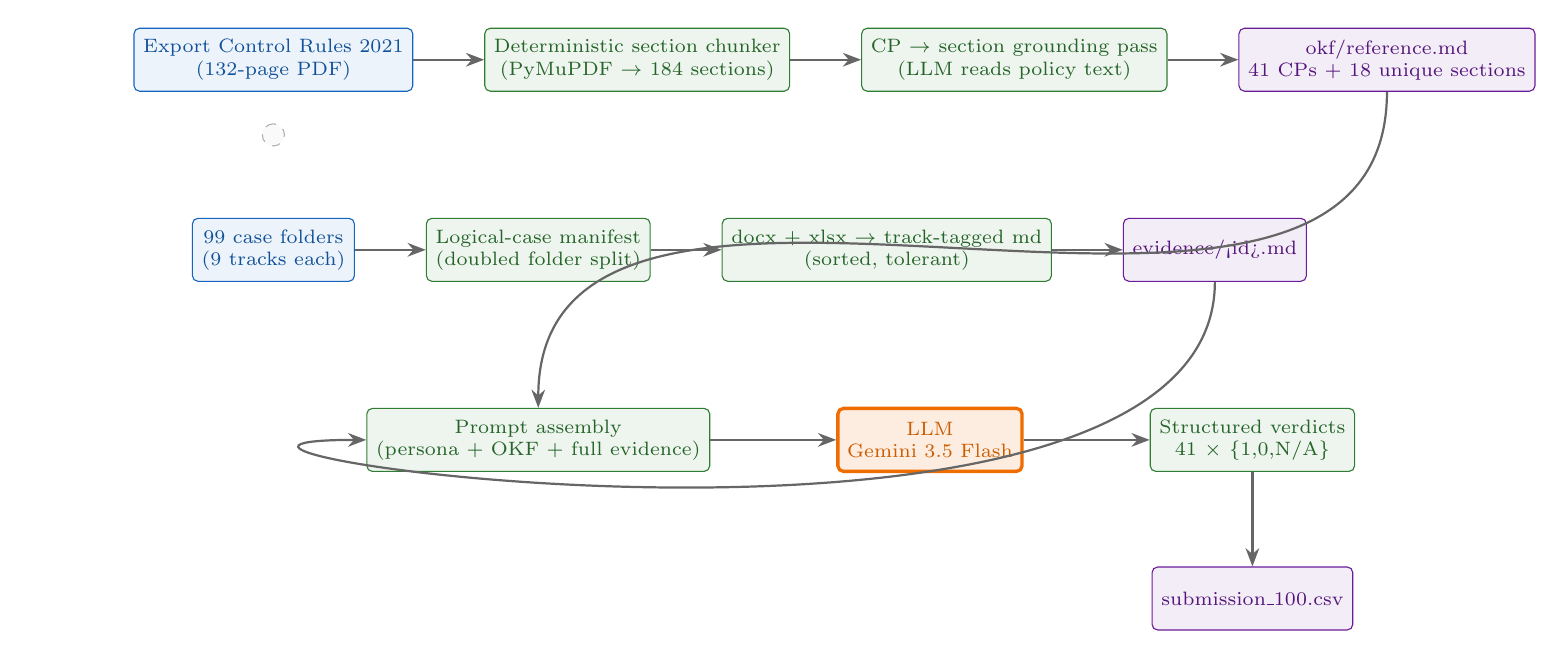
\begin{tikzpicture}[
  node distance=7mm and 8mm,
  box/.style={rectangle, rounded corners=2pt, draw, minimum height=8mm, align=center, font=\scriptsize},
  data/.style={box, fill=okfblue!8, draw=okfblue, text=okfblue!80!black},
  proc/.style={box, fill=procgreen!8, draw=procgreen, text=procgreen!80!black},
  llm/.style={box, fill=llmorange!12, draw=llmorange, very thick, text=llmorange!85!black},
  artifact/.style={box, fill=outpurple!8, draw=outpurple, text=outpurple!80!black},
  sub/.style={rectangle, rounded corners, draw=black!30, dashed, inner sep=4pt, fill=black!2},
  arr/.style={-{Stealth}, thick, black!60}
]
% Phase 1
\node[sub] (P1) at (0,0) {};
\node[data, above=4mm of P1.north] (pdf) {Export Control Rules 2021\\ (132-page PDF)};
\node[proc, right=9mm of pdf] (chunk) {Deterministic section chunker\\ (PyMuPDF $\to$ 184 sections)};
\node[proc, right=9mm of chunk] (map) {CP $\to$ section grounding pass\\ (LLM reads policy text)};
\node[artifact, right=9mm of map] (okf) {okf/reference.md\\ 41 CPs + 18 unique sections};
% Phase 2
\node[data, below=16mm of pdf] (raw) {99 case folders\\ (9 tracks each)};
\node[proc, right=9mm of raw] (man) {Logical-case manifest\\ (doubled folder split)};
\node[proc, right=9mm of man] (etl) {docx + xlsx $\to$ track-tagged md\\ (sorted, tolerant)};
\node[artifact, right=9mm of etl] (ev) {evidence/<id>.md};
% Phase 3
\node[proc, below=16mm of man] (asm) {Prompt assembly\\ (persona + OKF + full evidence)};
\node[llm, right=16mm of asm] (llm) {LLM\\ Gemini 3.5 Flash};
\node[proc, right=16mm of llm] (json) {Structured verdicts\\ 41 $\times$ \{1,0,N/A\}};
% Phase 4
\node[artifact, below=12mm of json] (csv) {submission\_100.csv};
% arrows
\draw[arr] (pdf)--(chunk); \draw[arr] (chunk)--(map); \draw[arr] (map)--(okf);
\draw[arr] (raw)--(man); \draw[arr] (man)--(etl); \draw[arr] (etl)--(ev);
\draw[arr] (okf.south) to[out=-90,in=90] (asm.north);
\draw[arr] (ev.south) to[out=-90,in=180] (asm.west);
\draw[arr] (asm)--(llm); \draw[arr] (llm)--(json); \draw[arr] (json)--(csv);
\end{tikzpicture}}
\caption{The four-phase FRECA architecture: Open Knowledge Format (OKF) bundle, deterministic evidence ETL, full-context LLM inference, and submission formatting. Blue = input data, green = deterministic process, orange = LLM, purple = output artifact.}
\end{figure}

\textbf{Design rationale.} Phase 1 (the \textbf{Open Knowledge Format}, OKF) maps each CP to its governing policy sections \emph{once}, offline --- this satisfies the no-hard-coding rule because the mapping is produced by an LLM reading the actual legislative text, not authored by hand. Phase 2 is pure, deterministic text extraction with \emph{zero compliance logic}. Phase 3 hands the \emph{full} evidence plus the \emph{relevant} policy text to the model in a single call. Phase 4 formats and validates.

\subsection{The Open Knowledge Format (OKF)}
The policy PDF is chunked into \textbf{184 section files} by a deterministic regex on section headers. A one-time LLM pass maps each of the 41 CPs to the section(s) that \emph{actually state} the obligation (not title-matches), producing YAML-cited bundle files. Deduplication collapses 64 citation instances into \textbf{18 unique sections} (4.31$\times$ reduction). The bundle is a committed, reproducible artifact, re-generated by \texttt{run\_cp\_mapping.py} via the API on demand.

\subsection{Deterministic Evidence ETL}
\texttt{ingest.py} flattens each case into a track-tagged markdown document, preserving table structure (the decisive signals live in \texttt{.xlsx} register rows) and tolerating missing tracks. A \textbf{logical-case manifest} splits the doubled folder into two cases, yielding exactly 100 logical cases.

\subsection{Full-Context Inference}
A single prompt carries the case's complete evidence ($\sim$8K words) plus the OKF bundle. The persona prompt enforces three evidence-handling disciplines learned from failure analysis: (1)~identity anchoring (per-track commodity/name fields are non-authoritative noise); (2)~boilerplate-vs-signal (fixed strings repeat across compliant and non-compliant cases; the status note is the real signal); (3)~N/A discipline (N/A only for an explicit, documented reason).

\section{Experiments and Ablations}

\subsection{Ablation A: Model selection}
\begin{table}[htbp]\centering\small
\caption{Full-context accuracy by model (10-case dev set).}
\begin{tabular}{@{}lrrr@{}}
\toprule
\textbf{Model} & \textbf{Accuracy} & \textbf{Tokens (10 cases)} & \textbf{Speed/case} \\
\midrule
Nemotron Ultra 550B & 314/410 = 76.6\% & 441K & $\sim$170s \\
DeepSeek V4 Pro & 334/410 = 81.5\% & 300K & $\sim$40s \\
\textbf{Gemini 3.5 Flash} & \textbf{353/410 = 86.1\%} & 442K & $\sim$90s \\
Sonnet 5 (Claude) & 373/410 = 91.0\% & $\sim$710K & $\sim$240s \\
\bottomrule
\end{tabular}
\end{table}

\begin{figure}[htbp]\centering
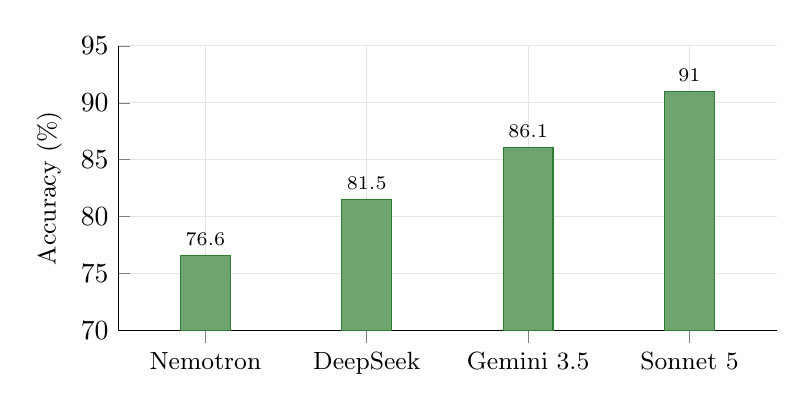
\begin{tikzpicture}
\begin{axis}[
  ybar, width=0.82\textwidth, height=5.2cm,
  symbolic x coords={Nemotron,DeepSeek,Gemini 3.5,Sonnet 5},
  xtick=data, x tick label style={font=\small, align=center},
  ymin=70, ymax=95, ylabel={Accuracy (\%)}, ylabel style={font=\small},
  nodes near coords, nodes near coords style={font=\scriptsize},
  bar width=18pt, axis lines*=left, ytick={70,75,80,85,90,95},
  grid=major, grid style={black!10}, enlarge x limits=0.18
]
\addplot[fill=procgreen!70, draw=procgreen] coordinates {(Nemotron,76.6) (DeepSeek,81.5) (Gemini 3.5,86.1) (Sonnet 5,91.0)};
\end{axis}
\end{tikzpicture}
\caption{Model bake-off: full-context accuracy on the 10-case dev set.}
\end{figure}

\textbf{Finding.} Gemini 3.5 Flash is the best reproducible-via-our-key model (+4.6pp over DeepSeek, +9.5pp over Nemotron), with a strong Element-4 edge (+16pp over Nemotron). Sonnet 5 is higher but was withdrawn from use.

\subsection{Ablation B: Model tier beats ensemble size}
Early experiments used a \textbf{3-persona ensemble} (Standard / Adversarial / Step-by-step at temperature 0) with majority-vote arbitration. A smaller base model (Haiku) in ensemble scored \textbf{70.7\%}, while a \emph{single} Sonnet pass scored \textbf{92.7\%} on the same case --- the ensemble could not compensate for a base model that skimmed past dense tabular registers. \textbf{Result: we dropped the ensemble in favour of one strong single pass.}

\subsection{Ablation C: Full-context vs hybrid RAG}
We built a complete hybrid-RAG branch: per-CP retrieval over evidence chunks with \textbf{BM25 (lexical) + bge-small dense (semantic) $\to$ weighted fusion $\to$ ColBERT late-interaction rerank $\to$ LLM}.

\begin{table}[htbp]\centering\small
\caption{Full-context vs hybrid RAG (10 cases).}
\begin{tabular}{@{}lrr@{}}
\toprule
\textbf{System} & \textbf{Accuracy} & \textbf{Tokens} \\
\midrule
Full-context (Gemini) & \textbf{86.1\%} & 442K \\
Hybrid RAG (best, $\alpha=1.0$) & 74.9\% & 610K \\
\bottomrule
\end{tabular}
\end{table}

\textbf{Finding.} RAG loses on \emph{both} axes. When the full evidence already fits one context window, retrieval only adds missed-signal risk (the decisive ``maintained in Mandarin'' sentence is retrievable only $\sim$56\% of the time) and per-call overhead.

\subsection{Ablation D: Hybrid fusion-weight grid search}
Measured purely on retrieval quality (track-hit@5 against gold), no LLM cost:

\begin{table}[htbp]\centering\small
\caption{Track-hit@5 vs dense weight $\alpha$ ($1-\alpha$ = BM25 weight).}
\begin{tabular}{@{}lccccc@{}}
\toprule
\textbf{dense model} & $\alpha{=}0$ (BM25) & 0.25 & 0.5 & 0.75 & 1.0 (dense) \\
\midrule
bge-small & 0.515 & 0.558 & 0.645 & 0.759 & \textbf{0.808} \\
bge-base & 0.515 & 0.547 & 0.580 & 0.659 & 0.726 \\
\bottomrule
\end{tabular}
\end{table}

\textbf{Finding.} Dense dominates --- \textbf{pure dense ($\alpha=1.0$) is optimal}, and the larger bge-base is \emph{worse} than bge-small (0.726 vs 0.808). This inverted the prior that ``higher BM25 weight is better.''

\subsection{Ablation E: Token/cost engineering}
\begin{table}[htbp]\centering\small
\caption{Pipeline cost evolution.}
\begin{tabular}{@{}lrrl@{}}
\toprule
\textbf{Version} & \textbf{Calls/case} & \textbf{Size} & \textbf{Outcome} \\
\midrule
v1 (per-element, per-persona) & 13 & $\sim$1.16M chars & unworkable \\
v2 (whole-case, 3 personas) & 3 & $\sim$215K tok & 84-agent bug \\
\textbf{v3 (single full-context)} & \textbf{1} & $\sim$44K tok & \textbf{final} \\
\bottomrule
\end{tabular}
\end{table}

Plus policy-text dedup (4.31$\times$), output-length caps via JSON Schema, and a \textbf{240s per-call timeout + per-case checkpointing} that made the 100-case run resilient to credit exhaustion and API hangs (3 mid-run recoveries, zero lost progress).

\subsection{Ablation F: Prompt engineering on planted signals}
The record-retention CP (CP38) was systematically wrong: the model read a \emph{constant} date-range string rather than the per-case \emph{status flag}. A single prompt rewrite (``the status note is the signal, not the target text'') took CP38 from \textbf{4/10 $\to$ 10/10} and lifted the aggregate 89.0\% $\to$ 91.0\% (Sonnet).

\section{Final Validation and Cross-Fold Results}

\subsection{Case-wise cross-fold (10-fold, leave-one-case-out)}
Using the 10-case dev set as validation folds, \textbf{Gemini 3.5 Flash} achieves mean accuracy \textbf{86.1\% $\pm$ 4.3\%} (min 80.5\%, max 95.1\%).

\subsection{Per-class metrics (competition definitions)}
With $\text{Precision}=\frac{TP}{TP+FP}$, $\text{Recall}=\frac{TP}{TP+FN}$, $F=\frac{2PR}{P+R}$:

\begin{table}[htbp]\centering\small
\caption{Per-class metrics on the 10-case dev set (Gemini 3.5 Flash).}
\begin{tabular}{@{}lrrrrr@{}}
\toprule
\textbf{Class} & \textbf{n} & \textbf{Precision} & \textbf{Recall} & \textbf{F} & \textbf{Per-class acc} \\
\midrule
1 (compliant) & 330 & 0.939 & 0.885 & \textbf{0.911} & 0.885 \\
0 (non-compliant) & 72 & 0.616 & 0.847 & \textbf{0.714} & 0.847 \\
N/A & 8 & 0.000 & 0.000 & \textbf{0.000} & 0.000 \\
\bottomrule
\end{tabular}
\end{table}

\textbf{Micro-accuracy = 86.1\% \quad Macro-F = 0.54 \quad Macro (average) accuracy = 0.58.}

\emph{Critical finding.} The competition's ``average accuracy'' is the \emph{mean of per-class accuracies}. Because our model never emits \texttt{N/A}, the N/A class has \textbf{0 recall}, dragging the macro score from 0.86 $\to$ 0.58. All 8 gold-N/A cells (the two Track-1-missing cases on CP1/2/6/7) were predicted \texttt{1}. \textbf{This --- not overall accuracy --- is the true optimisation target if the organisers score macro-averaged.}

\subsection{Per-element accuracy}
\begin{table}[htbp]\centering\small
\caption{Per-element accuracy (Gemini 3.5 Flash).}
\begin{tabular}{@{}lc@{}}
\toprule
\textbf{Element} & \textbf{Accuracy} \\
\midrule
Element-1 (registration/plans) & 85.7\% \\
Element-2 (buildings/facilities) & \textbf{98.9\%} \\
Element-3 (hygiene/waste/pest) & 85.8\% \\
Element-4 (traceability/phytosanitary) & 77.7\% \\
\bottomrule
\end{tabular}
\end{table}

\subsection{Full-corpus (100-case) production run}
\begin{itemize}[itemsep=2pt]
  \item \textbf{100/100 cases complete}, 0 blanks, 0 parse failures after hardening.
  \item Total cost: \textbf{4,493,869 tokens} ($\sim$44.9K/case).
  \item Output distribution: 3{,}118$\times$\texttt{1}, 982$\times$\texttt{0}, 0$\times$\texttt{N/A}.
  \item Resumed 4$\times$ across key changes and credit/rate-limit stops with zero lost progress.
\end{itemize}

\section{Reproducibility and Compliance}
\begin{itemize}[itemsep=2pt]
  \item \textbf{Pinned pipeline.} Canonical prompts, OKF bundle, and ETL are file-backed and content-addressed (MD5); a \texttt{--dry-run} mode verified byte-identical prompt hashes across runs.
  \item \textbf{API-only LLM usage.} All inference via the Lightning AI \texttt{litai} SDK (model string + key from environment, never hard-coded).
  \item \textbf{Determinism caveat.} Retrieval (BM25/dense/ColBERT) is deterministic ONNX; LLM inference is temperature-0 with a pinned model snapshot, but hosted inference carries residual run-to-run variance (documented in \texttt{HARDWARE\_AND\_DETERMINISM.md}).
  \item \textbf{OKF is re-derivable.} \texttt{run\_cp\_mapping.py} regenerates the CP$\to$section mapping via API; the mapping is model-dependent (12/41 CPs match across two models), so \emph{same model + prompt $\to$ same mapping} is the reproducibility contract.
\end{itemize}

\section{Conclusion and Future Work}
FRECA demonstrates that a \textbf{disciplined full-context LLM pipeline} --- grounded in a deduplicated knowledge bundle and hardened deterministic ETL --- achieves \textbf{86.1\% micro-accuracy} on a real-world compliance-audit task with full API-only reproducibility. The strongest ablations were \emph{negative results with high value}: ensembling a weak model and adding retrieval both \emph{hurt}, and the ``obvious'' BM25-heavy fusion prior was \emph{inverted} by the data. The single most important remaining risk is the \textbf{N/A-class scoring asymmetry} under macro-averaging; future work should (i)~teach the model to emit \texttt{N/A} when evidence is genuinely absent, and (ii)~re-validate against the organisers' exact scoring definition.

\end{document}
